\begin{figure}[H]
    \centering
    \begin{tikzpicture}
        \footnotesize

        \node at (0,2.4) (A) {Mesh division into sub-domains};

        \pause

        \draw[->] (0,2.05) -- (0,1.55);
        \node at (0,1.2) (B) {Choice of a \textbf{\textcolor{BrickRed}{local basis functions}}};

        \pause

        \draw[->] (0,0.85) -- (0,0.35);
        \node at (0,0) (C) {Exploitation of \underline{\textbf{compact support}}};

        \scriptsize

        \pause

        \node at (-3.458,-1.5) (D) {\textcolor{BrickRed}{$\bullet$} Leads to \textbf{sparse matrices}};
        \node at (-3.376,-2.25) (E) {\textcolor{BrickRed}{$\bullet$} Allows \textbf{local interpolation}};
        \node at (-3.174,-3) (F) {\textcolor{BrickRed}{$\bullet$} Enhances \textbf{numerical stability}};
        \node at (-3,-3.75) (G) {\textcolor{BrickRed}{$\bullet$} Enables \textbf{efficient parallelization}};

        \draw[->] (C) -- (-3.458,0) -- (D);

        \visible<4->{\node at (2.795,-2.58) (H) {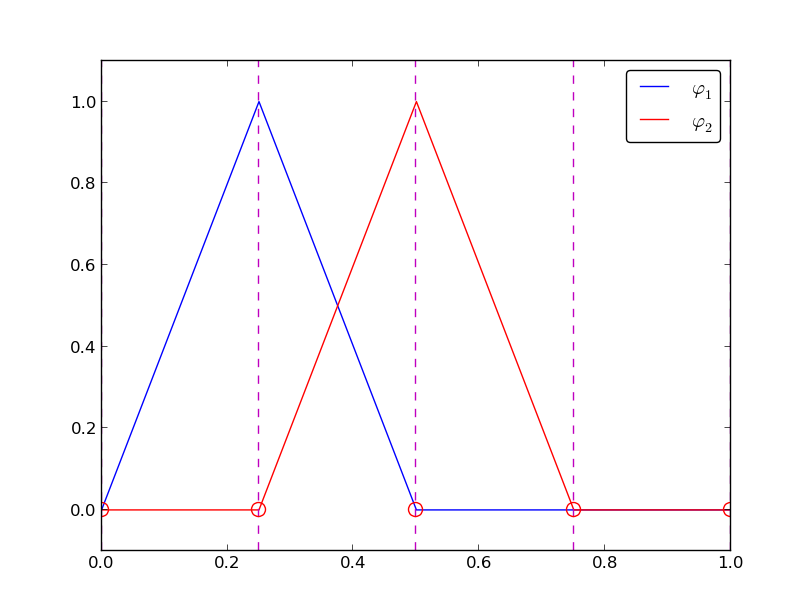
\includegraphics[width=0.45\textwidth]{Immagini/local-basis-functions.png}};}

        \normalsize
    \end{tikzpicture}
\end{figure}